\section{Interpolation des normales}
Comme nous pouvons le voir sur la \tsl{fig.\ref{fig:angel}}, l'utilisation
brute des
normales fournit par le modeleur ne nous permet pas d'obtenir un résultat très
esthétique. En effet, chaque face possède une normale et la transition entre
deux triangles est très marquée.\\

La solution consiste à assigner non pas une normale par face, mais 3 : une
pour chaque sommet. Ainsi, en moyennant la normale de chaque sommet en
fonction des faces auxquelles elle appartient, nous pourrons interpoler la
normale au point d'intersection en prenant maintenant en considération les
faces alentours. La \tsl{fig. \ref{fig:smoothnormal}}\ montre le résultat
obtenu.

\paragraph{Les coordonnées barycentriques}
\begin{wrapfigure}{r}{.5\textwidth}
  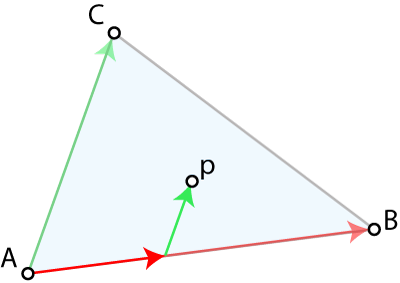
\includegraphics[width=.4\textwidth,
  keepaspectratio=true]{img/barycentricCoordinates}
  \label{fig:barycentric}
\end{wrapfigure}
Toute la difficulté de l'interpolation des normales repose donc sur la
pondération des différentes normales de la face. Pour cela, il est nécessaire
de passer en coordonnées barycentriques. Dans ce système, les coordonnées du
point d'intersection sont exprimées en fonction de deux côtés du triangle
comme le montre la \tsl{fig. \ref{fig:barycentric}}.\\

Il est alors évident de calculer le poids de chaque normal à la normal au
point d'intersection :
$$\vec{N} = N_a + a * (N_b - N_a) + b * (N_c - N_a)$$
où $a = |AB|$, $b = |AC|$ et $N_a$ (\resp $N_b$ et $N_c$) est la normale en
$A$ (\resp $B$ et $C$).

\subsection{Exemple}
\begin{figure}[h]
  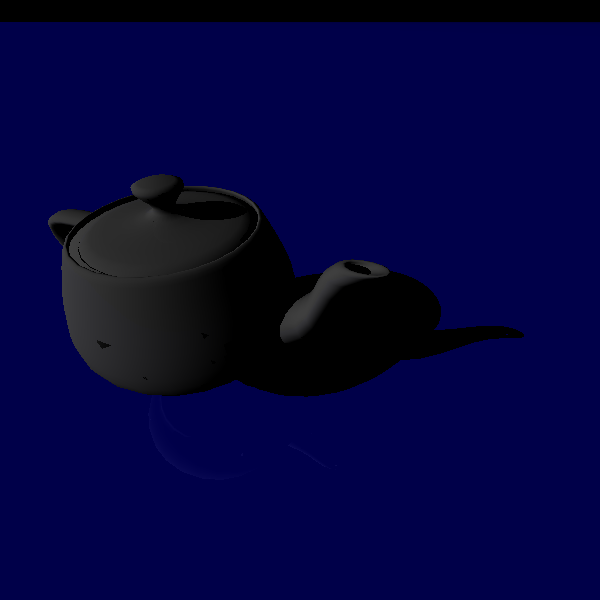
\includegraphics[width=\textwidth, keepaspectratio=true]{../../diary/16.png}
  \caption{Un exemple de rendu avec interpolation des normales\label{fig:smoothnormal}}
\end{figure}

\subsection{Amélioration}
\begin{description}
  \item [Génération des normales] Afin de réduire la complexité de
    l'importeur, j'ai laissé le calcul des normals par sommet à un programme
    externe. Il serait judicieux (et pas vraiment compliqué) d'intégrer le
    lissage au processus de chargement normal.
\end{description}

\subsection{Bug connu}
Aucun.
